
%\flushright{\hyperref[index]{\color{black!65}{Ritorna all'indice}}}\flushleft

	\section{A} \label{sec:A}

		\subsection{AMMINISTRATORE} \index{Amministratore} \label{amministratore}
		È uno dei \underline{\hyperref[ruoli]{ruoli}} in un progetto. In breve si occupa di controllare l'ambiente di lavoro. Nello specifico di:
		\begin{itemize}
			\item Amministrare le infrastrutture di supporto
			\item Risolvere problemi legati alla gestione dei processi
			\item Gestire la documentazione di progetto
			\item Controllare \underline{\hyperref[versione]{versioni}} e \underline{\hyperref[configurazione]{configurazioni}}
		\end{itemize}

		\subsection{\emph{ANALISI DEI REQUISITI}} \index{Analisi dei requisiti} \label{analisideirequisiti} %V.I
		L'attività di analisi dei \underline{\hyperref[requirements]{requisiti}} è lo step dopo lo studio di fattibilità (stesura documento \underline{\hyperref[studiofattibilita]{Studio di Fattibilità}}) e tratta sostanzialmente di capire appieno il problema.
		Riguarda la \underline{\hyperref[qualifica]{qualifica}} e se ne occupa l'\underline{\hyperref[analista]{Analista}} che deve cercare di entrare nell'ottica dell'utente. \\
		Lo \textit{svolgimento} dell'analisi prevede:
		 \begin{itemize}
			 \item Lo studio dei bisogni e delle fonti del dominio applicativo
			 \item Una prima classificazione dei requisiti
			 \item Una modellazione concettuale del sistema
			 \item L'assegnazione dei requisiti alle varie parti del sistema
			 \item La negoziazione con il committente
		 \end{itemize}
		Dopodiché avviene la redazione del \underline{\hyperref[pianoqualifica]{Piano di qualifica}} per metodi, tecniche, strumenti, tempi ecc. \\
		Le \textit{attività} di analisi sono:
			\begin{itemize}
				\item Studiare e definire il problema da risolvere, identificando il prodotto da commissionare, capendo cosa deve essere realizzato e definendo gli accordi contrattuali (compito del cliente)
				\item Verificare il costo e la \underline{\hyperref[qualita]{qualità}} in base ai requisiti derivanti dal cliente
				\item Studio dei bisogni e delle fonti, identificando, specificando e classificando i requisiti (lato fornitore)
				\item Modellazione concettuale del sistema con partizionamento in componenti (ambiti) a scopo di allocazione dei requisiti, per esempio con diagrammi d'uso (lato fornitore)
				\item Ripartizione dei requisiti a parti del sistema (lato fornitore)
				\item Accertare la soddisfacibilità dei requisiti rispetto ai vincoli di processo
				\item Assicurare, tramite \underline{\hyperref[tracciamento]{tracciamento}}, che i requisiti concordati siano tutti e soli quelli necessari (tutti i requisiti in AdR soddisfano un particolare bisogno) e sufficienti (tutti i bisogni rilevati nelle fonti sono requisiti in AdR)
				\item Determinare con il cliente l’utilità strategica dei requisiti concordati
				\item Adozione di norme redazionali (stesura documento \underline{\hyperref[norme]{Norme di Progetto}}), perchè aiuta a evitare espressioni ambigue, e glossario, perchè aiuta a garantire terminologia consistente
				\item Uso di metodi (semi-)formali, come diagrammi e formule, perchè aiuta a ridurre gli errori di interpretazione
			\end{itemize}
		I \textit{processi di supporto} implicati da esse sono:
			\begin{itemize}
				\item Documentazione, al fine di raccogliere i risultati dello studio di fattibilità e specificare i requisiti
				\item Gestione e \underline{\hyperref[manutenzione]{manutenzione}} dei prodotti, comprendente il \underline{\hyperref[tracciamento]{tracciamento}} dei requisiti, impostazione e gestione della configurazione e dei cambiamenti
			\end{itemize}
		All'interno del nostro progetto possiamo quindi dire di avere diversi prodotti documentali: per \textit{definire} i bisogni (utente e SW) abbiamo il \underline{\hyperref[capitolati]{capitolato d'appalto}}, per \textit{specificare} abbiamo appunto l'Analisi dei Requisiti (che è un documento contrattuale) e lo \underline{\hyperref[studiofattibilita]{Studio di Fattibilità}} (che è un documento interno del fornitore). \\
		Per la \textit{ripartizione} dei requisiti invece la questione è molto delicata perchè da qui inizia la \underline{\hyperref[progettazione]{Progettazione}}. Il confine tra Analisi e Progettazione è molto sottile: per esempio, l'Analista riesce già a vedere dei sotto-problemi che poi però sono compito del \underline{\hyperref[progettista]{Progettista}}.

		\begin{figure}[H]
			\centering
			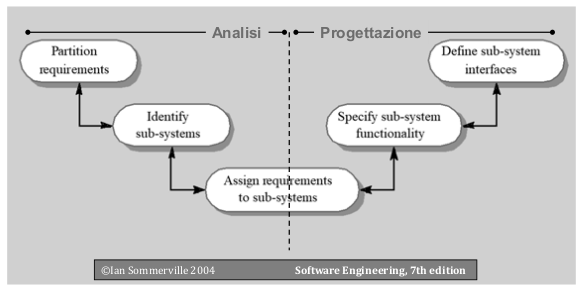
\includegraphics[width=0.8\textwidth]{img/conf}
			\caption{Confine tra Analisi e Progettazione.}
		\end{figure}

		Ci sono diversi approcci su come procedere per l'Analisi dei Requisiti:
			\begin{itemize}
				\item \textbf{\underline{\hyperref[topdown]{Top-down}}}
				\item \textbf{\underline{\hyperref[bottomup]{Bottom-up}}}
				\item \textbf{Agile}\label{agile}: generalmente parto da un'idea di una cosa che già esiste e penso alle funzionalità da poterci aggiungere. È una via di mezzo tra le altre due.
			\end{itemize}
		Le \textit{tecniche} di analisi comprendono:
			\begin{itemize}
				\item L'interazione con il cliente (il cui esito viene documentato in un verbale), tramite interviste o discussione di scenari
				\item Discussioni creative e collaborative, ovvero \underline{\hyperref[brainstorming]{brainstorming}}
				\item Prototipazione, interna (per il fornitore) o esterna (per la discussione con il cliente)
				\item La comprensione del dominio, che prevede:
				\begin{itemize}
					\item Una serie di domande base come \textit{A quali bisogni risponde il prodotto atteso?} e \textit{Quali problematiche d’uso esso comporta}
					\item L'acquisizione delle conoscenze tramite documentazione preesistente e interviste ai potenziali utenti
					\item Consolidamento del glossario che raccoglie e definisce i termini chiave del dominio per avere un'interazione ordinata con il committente
				\end{itemize}
			\end{itemize}
		Capita a volte che il progetto venga abbandonato e le principali cause sono:
			\begin{itemize}
				\item \underline{\hyperref[requirements]{Requisiti}} incompleti
				\item Insufficiente coinvolgimento del cliente e/o dell’utente (non sono necessariamente la stessa entità)
				\item Scarsità di risorse
				\item Attese irrealistiche
				\item Insufficiente competenza tecnologica e/o metodologica del fornitore
			\end{itemize}
		Mentre gli stati di progresso secondo \underline{\hyperref[semat]{SEMAT}} sono:
			\begin{itemize}
				\item \textit{Conceived}: il \underline{\hyperref[committente]{committente}} è identificato e gli \underline{\hyperref[stakeholder]{stakeholders}} vedono sufficienti opportunità per il progetto
				\item \textit{Bounded}:
				i macro bisogni sono chiari e i meccanismi di
				\underline{\hyperref[gestionerequisiti]{gestione dei requisiti}}
				(cambiamento e \underline{\hyperref[configurazione]{configurazione}}) sono fissati
				\item \textit{Coherent}: i requisiti sono classificati e quelli essenziali (obbligatori) sono chiari e ben definiti
				\item \textit{Acceptable}: i requisiti fissati definiscono un sistema soddisfacente per gli stakeholder
				\item \textit{Addressed}: il prodotto è pronto al rilascio e all'uso
				\item \textit{Fulfilled}: il prodotto merita la piena approvazione degli stakeholder tanto soddisfa i requisiti
			\end{itemize}
		Una struttura per il documento di Analisi dei Requisiti è definita dallo standard \underline{\hyperref[ieee830]{IEEE 830}}.


		%\subsection{ANALISI DEI RISCHI} \index{Analisi dei rischi} \label{analisirischi} %?

		\subsection{ANALISTA} \index{Analista} \label{analista}
		È uno dei \underline{\hyperref[ruoli]{ruoli}} in un progetto. Generalmente sono pochi ma hanno molta influenza sul successo del progetto. Conosce il dominio del problema e ha esperienza professionale, ma raramente segue il progetto fino alla consegna.

		\subsection{APPROCCIO} \label{approccio} \index{Approccio}
		Avvicinarsi/predisporsi. Può essere:
			\subsubsection{Sistematico} \label{sistematico}
			ovvero lavorando in maniera metodica, cioè ho un metodo da seguire che mi precede, e rigorosa usando ed evolvendo la \underline{\hyperref[best]{best practice}}.
			In questo è importante il tempo.
			\subsubsection{Disciplinato} \label{disciplinato}
			ovvero seguendo regole fissate.
			Per essere disciplinato ho bisogno di due documenti: Norme di Progetto per fissare il metodo, \underline{\hyperref[piano]{Piano di Progetto}} per sapere quando fare.
			\subsubsection{Quantificabile} \label{quantificabile}
			ovvero che permette di misurare \underline{\hyperref[efficienza]{efficienza}} ed \underline{\hyperref[efficacia]{efficacia}}. Il nostro fare deve produrre cose buone \textbf{oggettivamente}. Ci interessa misurare la qualità, per vedere il raggiungimento degli obiettivi che mi sono data.

		\subsection{ARCHITECTURE SELECTED}	\index{Architecture Selected}	\label{architectureselected}
		L'architettura viene capita e selezionata, oltre alla selezione delle tecnologie necessarie. \\
		È il primo degli stati di progresso del \underline{\hyperref[semat]{SEMAT}} per la \underline{\hyperref[progettazione]{progettazione}}.

		\subsection{ARCHITETTURA}	\index{Architettura} \label{architettura}
		Si intende architettura logica: è di alto livello (quindi non implementato, concettuale) e consiste nel dividere in parti per massimizzare il parallelismo. L'obiettivo è dividere fino a che non se ne trae più vantaggio, ovvero fino a che il costo della divisione diventa più un onere che un beneficio.
		Riporta UNA soluzione che soddisfa il cliente.
		Caratteristiche dell'architettura:
		\begin{itemize}
			\item Decomposta (suggerisce l'idea di top-down) in \underline{\hyperref[componente]{componenti}}
			\item Ha un'organizzazione: le componenti stanno insieme secondo regole date e ognuna ha un ruolo preciso e collabora
			\item Definisce le interfacce: qual è il modo in cui le componenti collaborano. Essa è associata a protocollo (= accordo) perché un'interfaccia si appoggia ad un protocollo
			\item Paradigmi (= come si fa) di composizione: componenti messe insieme secondo regole, limiti, vincoli. Definisce come vengono organizzate
		\end{itemize}
		Le architetture hanno scelte di paradigmi ed esistono più stili architetturali che determinano l'organizzazione dell'informazione di stato e l'interazione tra le parti. \\
		Le \underline{\hyperref[qualita]{qualità}} di una buona architettura sono: %slide 11/36
		\begin{itemize}
			\item \textbf{Modularità}: (legata a \underline{\hyperref[incapsulamento]{Incapsulamento}} e Disponibilità) ha l'obiettivo di minimizzare la dipendenza tra parti. Ha due opzioni:
			\begin{enumerate}
				\item Suddivide, come la pipeline è divisa in stadi
				\item In modo resiliente, ovvero facendo \textit{information hiding} altrimenti si espone ciò che è ``implementation detail'' (deve essere ben nascosto perchè altrimenti confonde e dà disagio)
			\end{enumerate}
			\item \textbf{Sufficienza}: deve soddisfare tutti i requisiti, coprire il bisogno
			\item \textbf{Comprensibilità}: deve essere capita dagli stakeholder, anche perché ci sono diversi stili
			\item \textbf{Robustezza}: sta in piedi anche se cambio un modulo
			\item \textbf{Flessibilità}: non deve collassare, deve essere in grado di evolvere (attuando modifiche a costo contenuto)
			\item \textbf{\underline{\hyperref[riuso]{Riusabilità}}}: fare nell'intento che possa essere buono anche per altri in futuro
			\item \textbf{Efficienza}: senza eccesso di risorse
			\item \textbf{Affidabilità}: quando c'è bisogno di utilizzarla, fa le cose che deve
			\item \textbf{Disponibilità}: sta in piedi senza grande bisogno di manutenzione (se una parte è sotto manutenzione, non deve essere interrotto tutto il sistema)
			\item \textbf{Sicurezza rispetto a malfunzionamenti}: \textit{``safety''}, non ho malfunzionamenti che fanno danno
			\item \textbf{Sicurezza rispetto a intrusioni}: \textit{``security''}, invulnerabile rispetto alle intrusioni. Mitigare il rischio e massimizzare i vantaggi
			\item \textbf{Semplicità}: le parti contengono solo il necessario, niente di superfluo
			\item \textbf{\underline{\hyperref[incapsulamento]{Incapsulamento}}}: (\textit{Information hiding}) l'interno delle componenti non è visibile dall'esterno, quindi i clienti conoscono solo l'interfaccia. Aumenta la manutenibilità e la possibilità di \underline{\hyperref[riuso]{riuso}}
			\item \textbf{\underline{\hyperref[coeso]{Coesione}}}: le parti che stanno insieme hanno gli stessi obiettivi e ognuna ha un ruolo
			\item \textbf{Basso accoppiamento}: l'accoppiamento è la nemesi della coesione, perchè quando viene mossa una parte ne viene conseguentemente mossa anche un'altra. Vogliamo quindi distinte parti che dipendono poco o niente le une dalle altre. È un probelma  però quando dall'esterno si fanno assunzioni su come certe cose stiano all'interno di altre e quando si condividono frammenti delle stesse risorse: bisogna cercare di massimizzare l'indice di utilità e minimizzare l'indice di dipendenza
		\end{itemize}
		%L'architettura definisce i ruoli.
		Tutte le qualità delle caratteristiche attese vanno perseguite e %slide 2/30 verifica e validazione
		tutto va sottoposto a verifica.

		\subsection{AUDIT PROCESS} \index{Audit Process} \label{audit}
		Imporre un andamento e assicurarsi che l'attività che si sta facendo si svolga nel migliore dei modi possibili. Permette di migliorare il \underline{\hyperref[way]{way of working}}. Si tratta di una revisione \textbf{esterna} (in particolare \underline{\hyperref[RR]{RR}} e \underline{\hyperref[RA]{RA}}).
